\chapter{Review of Classical Mechanics}
    \graphicspath{./figures}
    \section{The Hamiltonian}
 We have seen the \textbf{Hamiltonian} function in classical mechanics; resembling the energy of the dynamical system in study.\footnote{ recall that $H= T+V$}
 \begin{equation}
 H (\vec{p}, \vec{q}) \equiv \text{ Energy of the system}.
 \end{equation}
 Where, $\vec{p}$ and $\vec{q}$ are the generalised momentum and coordinates( configuration) for the system. We define the generalised/ canonical momentum as:\footnote{Note that $\vec{p}$ here is not always $m\vec{v}$ ! }
  \begin{equation}
  p_i = \dfrac{\partial \mathcal{L}}{\partial \dot{q}^i}.
  \end{equation}
  With $\mathcal{L}$ being the Lagrangian function.\footnote{ recall that $\mathcal{L}= T-V$}
    \subsection{Examples }
    \begin{enumerate}
    	\item The Hamiltonian for a free particle is given by: 
    	\begin{equation}
    	H = \frac{p^2}{2m}  
    	\end{equation}
    	\item In a central potential, the Hamiltonian takes the form :
    		\begin{equation}
    		H = \frac{p^2}{2m}  + g\; \frac{ Q_1 \, Q_2}{r}
    		\end{equation}
    		Where $g$ is a constant, called \textit{coupling constant}, and $ Q_1 \, Q_2$ are charges/ masses. Depending on the type of interaction.
    		\item A dipole in a magnetic field $B$ has the following Hamiltonian:
    			\begin{equation}
    			H = \vec{\mu} \cdot \vec{B}
    			\end{equation}
    		\item The Hamiltonian for a free rotating mass is: \footnote{ recall that $I = Mr^2$}
    			\begin{equation}
    			H = \frac{L^2}{2I}  
    			\end{equation}
    			Here, $L$ is the angular momentum of the system.
    		\item Lastly, a very important Hamiltonian, is the Hamiltonian for a simple harmonic oscillator ( SHO).
    				\begin{equation}
    				H = \frac{P^2}{2m}  + \frac{m \omega^2 \, q^2}{2} .
    				\end{equation}
    \end{enumerate}
    
    \section{Hamilton's equations}
   For a dynamical system with a Hamiltonian. The evolution of that system obeys the set of equations , known as \textbf{Hamilton's equations }:\footnote{ note that both $\vec{p}$ and $ \vec{q}$ are functions of time}
   \begin{align}
   \dfrac{\partial H}{\partial q^i} &= - \dot{p}_i \\
    \dfrac{\partial H}{\partial p_i} &=  \dot{q}^i 
   \end{align}
    Some dynamical systems however, does not obey these equations. These systems are known as\textit{ Hamiltonian constraint} systems.
    \subsection{ Poisson brackets}
    Let $f(\vec{q}, \vec{p})$, and $g(\vec{q}, \vec{p})$ be functions of both $\vec{q}$ and $\vec{p}$. One may define the following operation :
    \begin{equation}
    \{f,g\} \equiv \sum_i \left( \dfrac{\partial f}{\partial q^ i}\; \dfrac{\partial g}{\partial p_ i}-\dfrac{\partial g}{\partial q^ i}\; \dfrac{\partial f}{\partial p_ i}\right) 
    \end{equation}
    This operation is called \textbf{Poisson brackets}, it shall prove importance in quantisation, and also in understanding conserved quantities ( see homework). \\ It is interesting to Poisson bracket the Hamiltonian with components of $\vec{q}$ and $\vec{p}$, for example :
    \begin{align}
    \{q^j , H \} &= \sum_i  \dfrac{\partial q^ j}{\partial q^ i}\; \dfrac{\partial H}{\partial p_ i}-\dfrac{\partial H}{\partial q^ i}\;\underbrace{ \dfrac{\partial q^j}{\partial p_ i}}_{=0} \nonumber \\
    &= \sum_i \;  \delta^j_i \; \underbrace{\dfrac{\partial H}{\partial p_ i}}_{= \dot{q}^i} \nonumber\\
    &= \dot{q}^j
    \end{align} 
    Same goes for:
    \begin{equation}
    \{p_j, H\} =\dot{p}_j
    \end{equation}
    This actually leads us to the general result,  that for any function  $f(\vec{q}, \vec{p})$, we have:
     \begin{equation}
     \{f(\vec{q}, \vec{p}), H\} =\dfrac{\partial f(\vec{q}, \vec{p})}{\partial t}
     \end{equation}
     \section{Phase space}
     Since one only needs the $p$'s and $q$'s \footnote{ One needs as many of them as the number of degrees of freedom $f$ for the system} in order to fully describe the dynamical system. The \textbf{state} vector is defined in $2f$ dimensional space, called the phase space. 
    \begin{equation}
    \vec{S}(t) \equiv (\vec{q}(t), \vec{p}(t))
    \end{equation}
    \subsection{ Example: phase-space for SHO}
    This phase space for the SHO in 1-D is resembled by a circle:
    \begin{figure}[h!]
    	\centering
    	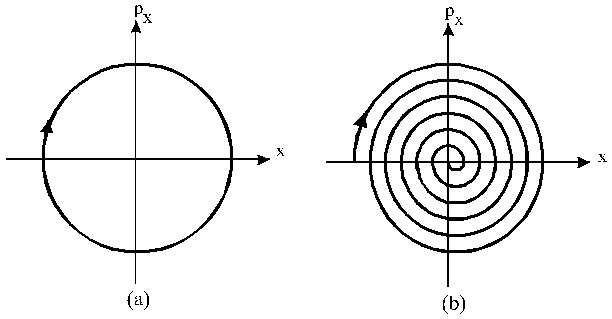
\includegraphics[scale=.4]{./figures/sho}
    	\caption{(a) The phase space for free SHO. (B) The phase space of a damped SHO}
    \end{figure}
    The circle resembles all the possible states the SHO can take, at any moment in time. In other words, this describes the full evolution of the system in time.\\Since energy is conserved for the free SHO, the system will keep being in the circle. As for damped one, when energy is lost. The system will spiral until it comes to a halt. 
    \section{Problems }
    \begin{enumerate}
\item Show that the Hamiltonian for a particle of mass $m$, orbiting a mass $M$, and they interact gravitationally is gien by:
    \begin{equation*}
    H = \frac{L^2}{2I}+ G \; \frac{M\, m}{r}
    \end{equation*}
    Then derive the equations of motion for this system, comment on your results.
    \item  Derive and solve the equation of motion for a 2-D SHO, with $ m=1$ and $ \omega =1$.
    \item  Show that :
    \begin{equation*}
    \{p_j , H\} = \dfrac{\partial p_j }{\partial t}
    \end{equation*}
 \item  Draw the shape of the phase space for a particle free-falling from altitude $y_0$

\item     Discuss conserved quantities, and Neother's theorem in light of Hamiltonian dynamics.  
    \end{enumerate}